\chapter{Marco Teórico}

La presente sección tiene como objetivo realizar una presentación ordenada de la literatura que respalde el trabajo realizado: para lo cual se divide en cuatro áreas principales tal y como se observa en la Figura \ref{marco}. En la Sección 2.1 se abordan conceptos generales eléctricos, específicamente los relacionados con los elementos utilizados en circuitos de potencia presentes en el radio que permita comprender la naturaleza del problema térmico que presenta el dispositivo. Para el caso de la Sección 2.2 se abordan aspectos relacionados con los métodos de modelado térmico que se pueden realizar, así como las consideraciones para la resolución del problema planteado. En la Sección 2.3 se trata lo referente a las consideraciones para la resolución del proyecto, también se presenta los aspectos propios del diseño de las soluciones termo-mecánicas pasivas debido a la relación bidireccional que presentan estos dos aspectos. 

\begin{figure}[H]
\centering
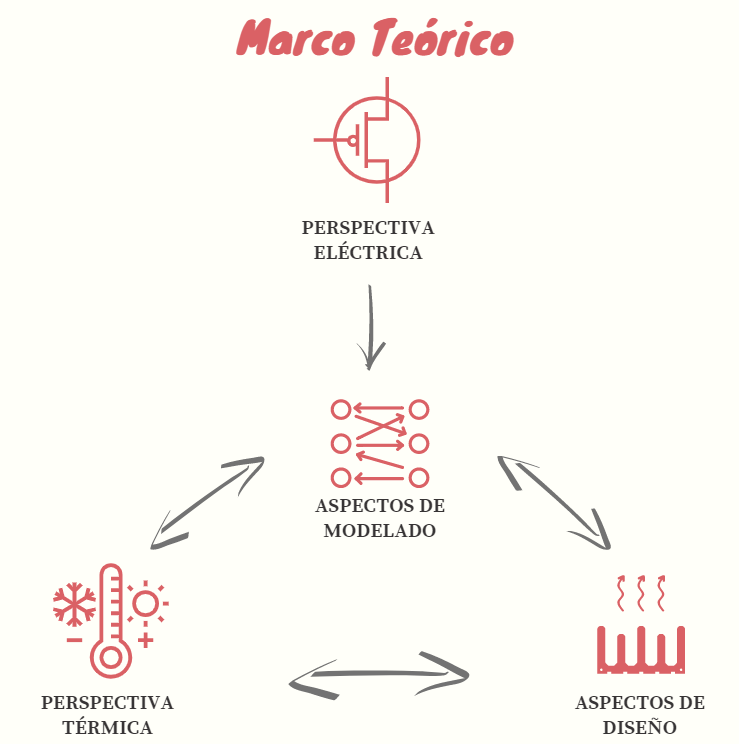
\includegraphics[scale=0.45]{Figuras/Marco_teorico.png}
\caption{Esquema de marco teórico}
Elaboración Propia
\label{marco}
\end{figure}


\section{Perspectiva Eléctrica}

Desde el siglo XIX, el físico inglés James Joule se dedicó al estudio de los efectos caloríficos producidos por el flujo de energía a través de diferentes medios; para lo cual realizó diferentes experimentos de los que obtuvo las siguientes conclusiones: \cite{joule}

\begin{enumerate}
    \item En un conductor, el flujo de la corriente eléctrica produce calentamiento.
    \item El incremento en la temperatura debido al flujo de corriente a través de un conductor, es proporcional al tiempo que dure dicho flujo de corriente.
    \item El aumento de la temperatura varía en relación con la intensidad de la corriente.
    \item El calentamiento es proporcional a la resistencia del conductor.
\end{enumerate}

Basado en estas observaciones postuló la siguiente Ley \cite{joule}:

\begin{center}

\centering
\textit{ La cantidad de calor producido por un conductor eléctrico es directamente proporcional al cuadrado de la intensidad ($I^2$), al valor de la resistencia del conductor y al tiempo, en segundos, durante el cual circule la corriente.}

\end{center}

Los dispositivos eléctricos, principalmente los de potencia, no escapan de los principios de esta ley, por lo que el aumento de temperatura debido a los flujos de corrientes que manejan, los ciclos de trabajo a los que son sometidos y el rápido avance de la tecnología junto con la necesidad de sistemas más eficientes y económicos, han tenido un impacto especialmente reflejado en el tamaño de los componentes electrónicos, además han provocado que la comprensión de la transferencia de calor en la cual se estudia el punto de equilibrio del medio continuo pierda validez a nano-escala, y el tamaño del dispositivo, junto con el tiempo pasen a ser determinantes como sucede en el caso de los IGBT y los MOSFET. \cite{cengel} 

\subsection{Semiconductor:}

Estos elementos pueden realizar la función de conductor o aislante de una manera selectiva según condiciones externas como campos electromagnéticos, campos eléctricos y radiación que determinan si dicho elemento se comporta como un circuito abierto o como un circuito cerrado. Dentro de los posibles elementos utilizados para la fabricación de semiconductores los más utilizados por la industria de componentes eléctricos son el Silicio (Si) y el Germanio (Ge) a los cuáles se les introduce partículas de otros elementos para convertirlos en semiconductores.\cite{beltran}
\\
Según el tipo de impureza que se introduzca, se puede obtener: 

\begin{itemize}
    \item Tipo N: poseen impurezas pertenecientes al grupo Va (Fósforo) lo que se traduce en un excedente de electrones libres.
    \item Tipo P: Sus impurezas son pertenecientes a compuestos del grupo Illa (Cadmio, Boro, entre otros) lo que provoca, debido a la falta de electrones, un exceso de cargas positivas.
\end{itemize}

En ambos casos el componente semiconductor es el encargado de realizar la conmutación de la señal eléctrica y existen dos principales tipos, el transistor unipolar o conocido por sus siglas en ingles FET (field-effect-transistor) y el transistor bipolar; su diferencia radica en que para el primero la activación del terminal de control se realiza aplicando tensión entre la puerta y la fuente, mientras que en el segundo se realiza inyectando corriente en la base que regula la conmutación.

\subsection{Tipos de semiconductores}

\textbf{MOSFET:} Su nombre proviene del acrónimo en ingles Metal-oxide-semiconductor-field-effect y su principio de funcionamiento consiste en aplicar tensión en la puerta (Gate) para que los electrones se muevan a la parte de abajo en la zona n+ en donde la tensión provoca que se genere un flujo de electrones que une las dos zonas conductoras llamadas fuente (Source) y Drenaje (Drain), para permitir el paso de la corriente \cite{beltran}. En la  Figura \ref{tipo n} se observa como, cuando se aplica un voltaje en la compuerta mayor a \SI{0}{\volt} y mayor que el voltaje de umbral se establece un puente de electrones entre la compuerta fuente y la compuerta de drenaje.

Los MOSFET son utilizados en aplicaciones de bajo voltaje ($<$\SI{250}{\volt}), baja potencia y altas frecuencias ($>$ \SI{200}{\kilo\hertz}), esto debido a la forma en que tienen pérdidas, tema que se tratará más adelante; sin embargo, se debe mencionar que en el caso de los MOSFET, las principales pérdidas  se deben a conducción y/o conmutación, estas últimas son las más bajas. \cite{beltran}

\begin{figure}[H]
\centering
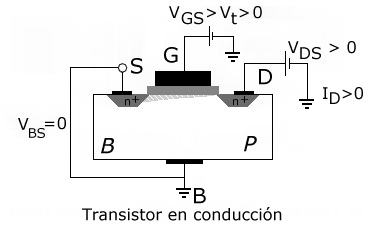
\includegraphics[scale=1]{Figuras/mosfet.png}
\caption{MOSFET tipo N en estado de conducción}
Fuente: \cite{Imagen_mosfet}
\label{tipo n}
\end{figure}

\textbf{BJT:} Utilizados principalmente en amplificadores los transistores de unión bipolar tienen un funcionamiento similar al MOSFET con la principal diferencia de que en este caso la conmutación se realiza al inyectar corriente en la base. Otra característica es que se encuentran construidos por tres piezas semiconductoras las cuales se disponen en dos posibles configuraciones: NPN o PNP . 

\begin{figure}[h]
\centering
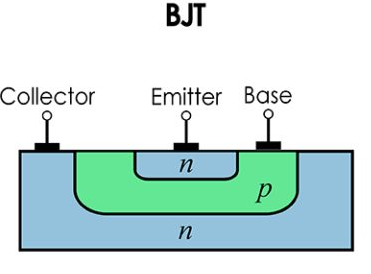
\includegraphics[scale=0.7]{Figuras/bjt.png}
\caption{BJT tipo NPN}
Fuente: \cite{bjt}
\label{bjt}
\end{figure}

\textbf{IGBT:} La interpretación del acrónimo es Insulated-gate bipolar transistor. Su principio de funcionamiento es similiar al de un MOSFET con la diferencia de que en este caso se agrega una capa p+ adicional la cual inyecta huecos en la capa n- y provoca una reducción en la caída de voltaje en la conducción; esto es motivo de reducción de las pérdidas por el mismo motivo, en consecuencia, son utilizados en aplicaciones de alto voltaje ($>$\SI{1000}{\volt}), bajas frecuencias en conmutación ($<$\SI{20}{\kilo\hertz}) y alta potencia. Sus características de construcción no permiten la conducción de corriente en modo inverso, por lo que a diferencia de otros transistores no requiere de un diodo intrínseco.\cite{beltran}

\begin{figure}[h]
\centering
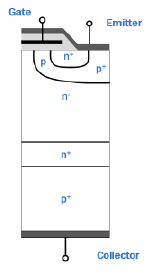
\includegraphics[scale=0.9]{Figuras/igbt.png}
\caption{IGBT tipo n}
Fuente: \cite{beltran}
\label{igbt}
\end{figure}

\subsection{Pérdidas en Semiconductores:}

En esencia los transistores son interruptores dentro de un circuito de potencia, por lo que se presentan pérdidas cuando el transistor se encuentra en estado de conducción y pérdidas cuando el mismo realiza la conmutación entre un estado y otro.

\textbf{Pérdidas por Conmutación:} Como su nombre lo sugiere estas pérdidas se dan en el momento en que el componente se apaga y enciende, produciéndose dichas pérdidas en el lapso que el componente tarda en responder al pasar de un estado a otro.\cite{beltran} 

\begin{figure}[h]
\centering
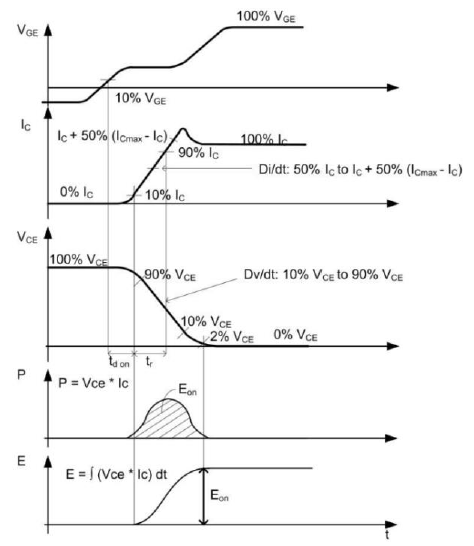
\includegraphics[scale=0.65]{Figuras/on.png}
\caption{Transistor en transición de encendido}
Fuente: \cite{beltran}
\label{encendido}
\end{figure}

Tal y como se observa en la Figura \ref{encendido} la energía que se pierde durante la conmutación de encendido del componente se cuantifica desde el momento que se da un flujo del \SI{10}{\percent} de la corriente de conducción hasta llegar a un \SI{90}{\percent} de la misma.   

\begin{figure}[H]
\centering
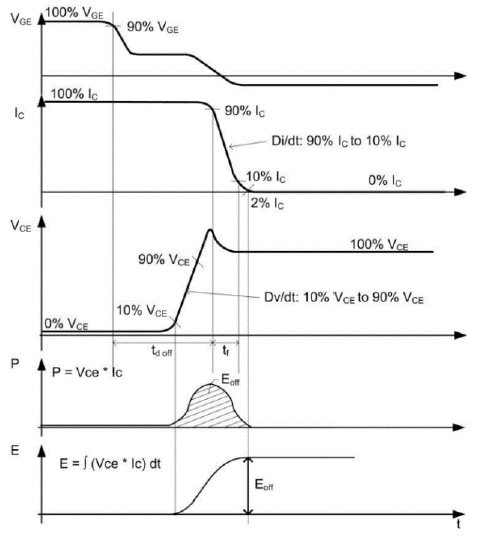
\includegraphics[scale=0.65]{Figuras/off.png}
\caption{Transistor en transición de apagado}
Fuente: \cite{beltran}
\label{apagado}
\end{figure}

Para el caso del estado transitorio de apagado en la Figura \ref{apagado} se observa que el tiempo que se considera para el cálculo de la pérdida de energía se cuenta desde el momento en que la caída de tensión representa un \SI{10}{\percent} del valor nominal hasta el momento en que la corriente de conducción alcanza un \SI{2}{\percent} de su valor nominal.

\textbf{Pérdidas por Conducción:} Se define como la energía disipada en forma de calor durante el tiempo en el que el componente, en este caso el transistor, se encuentra en estado de conducción \cite{beltran}. En este punto es importante resaltar que dichas pérdidas de potencia se pueden relacionar con la temperatura de unión como se muestra en la Ecuación \ref{pconduccion}, en donde las pérdidas por conducción son una función dependiente de la corriente de conducción y la temperatura de junta.

\begin{equation}\label{pconduccion}
    P_{cond} = f(I_{c},T_{j})  
\end{equation}

\section{Perspectiva de Modelado}

Una definición formal de modelo es la de ``esquema teórico, por lo general de carácter matemático, de un sistema o de una realidad compleja, que se elabora para facilitar su comprensión y el estudio de su comportamiento"\cite{rae}. En otras palabras un modelo es una forma de representación simplificada de la realidad o bien de un problema complejo que requiere de análisis, el cual por lo general se realiza a través de lenguaje matemático. Ahora bien en el momento que dicho lenguaje matemático es utilizado para describir un fenómeno o situación de naturaleza no matemática es donde se introduce el término de modelo matemático. \cite{morten}

Los modelos como tales pueden tener dos propósitos generales, uno de carácter descriptivo y otro de carácter predictivo, este último es mucho más complicado epistemológicamente ya que implícitamente requiere de supuestos o hipótesis que relacionen dos situaciones  diferentes pero con ciertas similitudes que los correlaciona: por un lado la situación que estima las características propias del fenómeno y por otro relacionan los condicionantes que permiten predecir el comportamiento de futuras situaciones. En el caso de un modelo descriptivo, si bien es cierto implica la definición de las características propias del fenómeno, dicha información es utilizada para análisis de un hecho ya ocurrido con diferentes propósitos. \cite{morten} 

Desde un punto de vista general, la literatura describe una serie de flujo de procesos para la realización de un modelo matemático, y aunque ciertas etapas del proceso varían el orden a seguir entre un autor y otro, se pueden resumir las etapas de la siguiente manera: \cite{morten}, \cite{comillas}

\begin{enumerate}
    \item Formulación del problema: Trata de la recolección y análisis pertinente de la información relevante que defina de una manera más precisa la situación que se requiere resolver, en este punto es donde también se plantean los supuestos y se recolectan los datos que más adelante deberán ser validados.
    \item Sistematización y formulación matemática: Consiste en la selección de las relaciones y objetos relevantes en el dominio de la investigación de manera tal que permita realizar una idealización del problema cuando se establecen las variables, parámetros y ecuaciones matemáticas que describen el problema
    \item Resolución: Hace uso de métodos matemáticos mediante la implementación de un algoritmo de obtención numérica óptima o cuasi-óptima con el objetivo de llegar a resultados matemáticos y conclusiones.
    \item Evaluación de la validez del modelo por comparación de datos: En este punto los resultados obtenidos de la resolución se deben comparar con los datos observados o predichos, con el conocimiento teórico o con la experiencia personal o compartida sin embargo, se debe aclarar que en el caso (el ideal) de validar el modelo en comparación con datos, los mismos no pueden ser los utilizados para la construcción del modelo ya que la intención de esta etapa, como su nombre lo indica, es determinar la utilidad del modelo para la descripción del fenómeno.
    \item Interpretación de los resultados y conclusiones: Una vez se tiene un modelo válido, del mismo se puede obtener información que permita sacar conclusiones y tomar decisiones respecto al fenómeno o situación estudiada según los propósitos planteados en la identificación del problema. 
    \item Implantación, documentación y mantenimiento: Esta etapa implica un cierre del ciclo de modelado, en el cual, una vez se tienen los resultados óptimos del modelo, la documentación necesaria permanece para garantizar la amplia difusión del modelo, así como sus posteriores correcciones.
\end{enumerate}

Es importante aclarar que las etapas antes descritas, lejos de ser un proceso lineal, son un constante ciclo en donde un modelo o sistema matemático se va adaptando a la interpretación del mundo real, en última instancia son el problema y la comprensión del mismo en la realidad los que definen los pasos a seguir para realizar un modelo que lo represente \cite{morten}. Por otro lado los pasos 4 y 5 suelen ser un motivo de discrepancia entre los autores ya que según la literatura consultada, dichas etapas suelen encontrarse invertidas, realizándose una interpretación de los resultados antes de la validación, pero como ya se mencionó la naturaleza misma del modelo determinará el orden de las etapas.

Es por ello que existen múltiples técnicas de modelado, mas aún con las herramientas de programación y software CAD 3D que permiten realizar modelos matemáticos de gran complejidad. En el caso de dispositivos electrónicos existe amplia literatura que describe diferentes tipos de modelos que caracterizan el comportamiento térmico de estos dispositivos a través de circuitos RC equivalentes. Los arreglos más comunes son las redes de Cauer y Foster. \cite{realtime}

\begin{figure}[H]
\centering
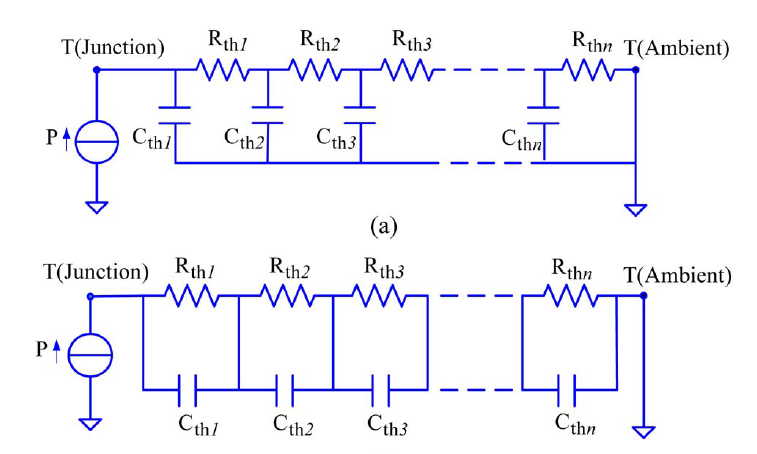
\includegraphics[scale=0.65]{Figuras/foster.png}
\caption{Red de Cauer y Foster respectivamente}
Fuente: \cite{realtime}
\label{foster}
\end{figure}

En la Figura \ref{foster} se observan dos configuraciones típicas que permiten simular un dispositivo de potencia  para determinar la temperatura de unión; en el caso de la red de Cauer describe el comportamiento térmico a lo largo de las capas constructivas del dispositivo, pero tiene la desventaja de tener una compleja implementación; por otro lado la red de Foster es de fácil implementación sin embargo, no predice el comportamiento térmico de sus capas constructivas. \cite{realtime}

Tomando como referencia la red de Foster, se puede obtener una impedancia térmica del sistema tal y como se muestra:

\begin{equation}\label{2}
    Z_{th}(t)=\sum ^{n}_{i=1}R_{i}\left ( 1-e\frac{t}{R_{i}C_{i}} \right )
\end{equation}

Donde $Z_{th}(t)$ es a lo que se conoce como  impedancia térmica, $R_{i}$ y $C_{i}$ son las resistencia y capacitancia térmica respectivamente de cada nodo de la red de Foster (figura \ref{foster}). La obtención de $Z_{th}(t)$ se puede realizar mediante una curva de mejor ajuste para obtener los valores de  $R$ y $C$  por medio de un software y con datos obtenidos a través de la experimentación. \cite{alfaro} 

\subsection{Red Generalizada}

Por otra parte, la Figura \ref{foster}  permite introducir el concepto de red generalizada, la cual es una extensión de las propiedades y teoremas de las redes eléctricas mediante la interconexión de elementos y fuentes generalizadas; para lo cual se utilizan  los conceptos de transvariable \( (\upsilon) \) y pervariable (f), donde la transvariable  requiere de dos puntos para medirse y se obtiene a través de los elementos, mientras que la pervariable se propaga por los elementos y su medición solo requiere de un punto. \cite{alfaro} 

Lo antes descrito se puede representar gráficamente de la siguiente manera:

\begin{figure}[H]
\centering
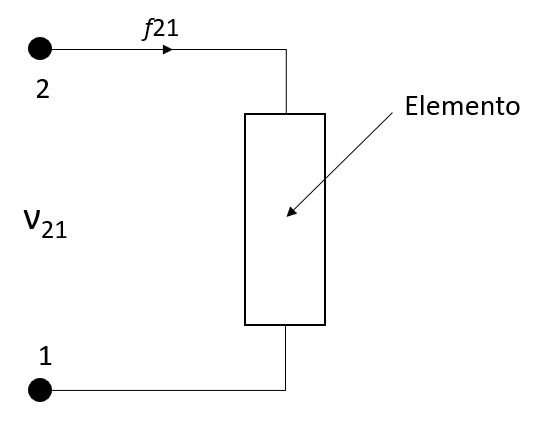
\includegraphics[scale=0.45]{Figuras/red.png}
\caption{Esquema de la Red Generalizada}
Fuente: Elaboración propia
\label{red}
\end{figure}


Por lo que el flujo de potencia que entra desde el punto 2 hacia el 1 se describe como \cite{alfaro}:

\begin{equation}\label{3}
    P(t) = f_{21}(t)\cdot \upsilon _{21}(t)
\end{equation}

En la Figura \ref{red} el ``Elemento'' adquiere su respectivo equivalente generalizado, dentro del circuito según se requiera para describir el sistema, como por ejemplo, puede ser reemplazado por un resistor generalizado, capacitor generalizado o bien incluso tener una fuente ideal de pervariable o transvariable. Para el caso de los sistemas térmicos se presentan a continuación los conceptos equivalentes dentro de la red generalizada:

\begin{table}[H]
\centering
\caption{Elementos generalizados para la representación de sistemas térmicos \cite{alfaro}}
\label{tab:2}
\begin{tabular}{@{}ccccc@{}}
\toprule
\textbf{\begin{tabular}[c]{@{}c@{}}Pervariable\\ ($f$)\end{tabular}} &
  \textbf{\begin{tabular}[c]{@{}c@{}}Integral de\\ Pervariable\\ ($h$)\end{tabular}} &
  \textbf{\begin{tabular}[c]{@{}c@{}}Transvariable\\ ($\upsilon$)\end{tabular}} &
  \textbf{\begin{tabular}[c]{@{}c@{}}Capacitor \\ Generalizado\\ ($C_{g}$)\end{tabular}} &
  \textbf{\begin{tabular}[c]{@{}c@{}}Resistor \\ Generalizado\\ ($R_{g}$)\end{tabular}} \\ \midrule
\begin{tabular}[c]{@{}c@{}}Flujo de calor\\ ($q$)\end{tabular} &
  \begin{tabular}[c]{@{}c@{}}Calor \\ ($H$)\end{tabular} &
  \begin{tabular}[c]{@{}c@{}}Diferencia de\\ Temperatura\\ ($\Delta T$)\end{tabular} &
  \begin{tabular}[c]{@{}c@{}}Capacitor \\ Térmico\\ ($C_{t}$)\end{tabular} &
  \begin{tabular}[c]{@{}c@{}}Resistor \\ Térmico\\ ($R_{t}$)\end{tabular} \\ \bottomrule
\end{tabular}
\end{table}

\subsubsection{Función de Transferencia}

Se define como una expresión matemática que relaciona y caracteriza una condición de entrada $u(t)$ con una condición de salida $y(t)$ en donde ambas están relacionadas mediante una ecuación diferencial para un sistema o proceso en específico. \cite{transferencia}

\begin{equation}\label{4}
    a_{0}y(t)+ a_{1}\frac{dy(t)}{dt}+\cdots+a_{n}\frac{d^{n}y(t)}{dt}=b_{0}u(t)+b_{1}\frac{du(t)}{dt}+\cdots +b_{n}\frac{d^{n}u(t)}{dt}
\end{equation}
\\
Representado a manera de bloques queda tal y como se muestra a continuación, donde se logra apreciar que la salida es dependiente de la entrada:

\begin{figure}[H]
\centering
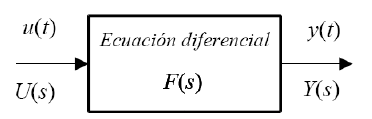
\includegraphics[scale=0.8]{Figuras/f.png}
\caption{Diagrama de entrada y salida de un sistema}
Fuente:\cite{transferencia}
\label{trans}
\end{figure}

Para lograr obtener la función de transferencia se recurren a las transformadas de Laplace, la cual es muy utilizada en aplicaciones ingenieriles en donde se presentan problemas con discontinuidades, o bien el comportamiento del sistema es periódico pero no fácilmente describible mediante expresiones matemáticas comunes.
\begin{equation}\label{laplace}
    F(s)=\pounds (f)=\int_{0}^{\infty }e^{-st}f(t)dt
\end{equation}

La transformada de Laplace básicamente consiste en tomar una ecuación diferencial y transformar cada derivada en un simple producto por $s$ y a la ecuación diferencial en $t$, en una ecuación algebraica en cuestión del termino complejo $s$ que define los polinomios: \cite{transferencia}

\begin{equation}\label{poli1}
    A(s)=\sum_{i=0}^{\infty }a_{i}s^{i}
\end{equation}

\begin{equation}\label{poli2}
 B(s)=\sum_{i=0}^{\infty }b_{i}s^{i}
\end{equation}

Por lo que, si se observa la Figura \ref{trans}, una vez que se obtienen las transformadas de ambos miembros de la ecuación se tiene que:

\begin{equation}
    Y(s)A(s) = U(s)B(s)
\end{equation}

Si se coloca la salida como la entrada multiplicada por el cociente de los polinomios \ref{poli1} y \ref{poli2}, donde a dicho cociente se le conoce como función de transferencia $F(s)$: \cite{transferencia}

\begin{equation}
    Y(s)A(s) = U(s)F(s)
\end{equation}

Donde:
\begin{equation}
F(s)=\frac{B(s)}{A(s)}
\end{equation}

Ahora bien, para utilizar el método se debe tener en consideración lo siguiente:\cite{transferencia}

\begin{itemize}
    \item La función de transferencia es aplicable exclusivamente a sistemas lineales e invariantes en el tiempo, por lo que en ocasiones se requiere de una linealización previa para implementar el método. Para que un sistema sea lineal, es importante recordar que debe cumplir con el principio de superposición y homogeneidad.
    \item En una función de transferencia el numerador es de orden menor o igual al del denominador, lo cual sucede siempre en sistemas físicos y se asumirá de manera implícita.
    \item A las raíces del denominador ($A(s)$) se le conocen como polos y estos determinan la estabilidad de la función; por otra parte a las raíces del numerador ($B(s)$) se le denominan ceros de $F(s)$.
    \item Sistemas que son físicamente distintos pueden tener la misma función de transferencia es decir, la función de transferencia caracteriza la dinámica del sistema, mas no proporciona información respecto a la estructura física real del sistema. 
\end{itemize}

\section{Perspectiva Térmica y de Diseño}
\textbf{Transferencia de Calor:} Se define como el proceso de propagación de calor en distintos medios, este se produce siempre que existe un gradiente térmico o cuando dos sistemas con temperatura diferente se ponen en contacto. El equipo de transferencia de calor, como los intercambiadores de calor están diseñados tomando en cuenta el análisis de la transferencia de calor. Los problemas de esta ciencia que se encuentran en la práctica se pueden considerar en dos grupos: 1) de capacidad nominal y 2) de dimensionamiento. Los problemas de capacidad nominal tratan de la determinación de la razón de la transferencia de calor, para un sistema existente a una diferencia específica de temperatura. Los problemas de dimensionamiento tratan con la determinación del tamaño de un sistema con el fin de transferir calor a una razón determinada para una diferencia específica de temperatura. \cite{cengel}

\textbf{Calor:} Se define como la forma de energía que se puede transferir de un sistema a otro como resultado de un diferencial de temperatura. \cite{cengel} 

\textbf{Calor Sensible:} Es la parte de la energía interna de un sistema asociada con el grado de actividad que sus moléculas tengan, entre mayor sea esta actividad mayor será el incremento de temperatura \cite{cengel}. También es el calor asociado a los cambios de temperatura de bulbo seco y dentro de las cargas térmicas que representan este tipo de energía interna, están las luces, componentes y dispositivos electrónicos así como motores eléctricos. \cite{apc}

\textbf{Calor Latente:} Esta asociado a la energía potencial interna de un sistema, por ende, hace referencia a la energía interna necesaria para vencer las fuerzas intermoleculares, lo que puede implicar cambios de fase \cite{cengel}. Por otra parte este calor se relaciona con la cantidad de humedad contenida en un cuerpo. \cite{apc}

\textbf{Mecanismos de transferencia de calor:} Existen tres mecanismos básicos.\cite{cengel}

\begin{itemize}
    \item Conducción: Transferencia de energía de las partículas más energéticas de una sustancia hacia las adyacentes, menos energéticas, como resultado de la interacción entre ellas.
    \item Convección: Transferencia de calor entre una superficie sólida y el líquido o gas adyacente que está en movimiento; y comprende los efectos combinados de la conducción y del movimiento del fluido
    \item Radiación: La energía emitida por la materia en forma de ondas electromagnéticas (o fotones), como resultado de los cambios en las configuraciones electrónicas de los átomos o moléculas.
\end{itemize}

\textbf{Convección natural:} Cuando la velocidad del fluido que está asociado a la transferencia de calor suele ser menore a \SI{1}{\meter/\second}, se habla de convección natural; en estos casos el coeficiente de transferencia por convección como está relacionado con la velocidad del fluido, suele ser muy bajo en comparación con los coeficientes de convección forzada. En estos casos  la diferencia de temperatura entre el medio y el objeto provoca transferencia de calor, por consiguiente, la temperatura del objeto decaerá un tanto y el fluido aumentará su temperatura en un tanto; esto provoca el efecto de flotación en donde la capa fina de aire que cubre el objeto caliente y que aumenta su temperatura, cambiará su densidad y se desplazará hacia las capas exteriores del fluido, el aire con una densidad menor y por ende una temperatura menor reemplazará la capa de aire caliente que se desplazó. Este proceso implica un movimiento del fluido y se repetirá hasta que el objeto caliente se encuentre en equilibrio térmico con el fluido. \cite{cengel}

\textbf{Convección natural sobre superficies:} Depende de la orientación y forma geométrica de la superficie, así como de las propiedades termofísicas del fluido. La resolución de problemas de convección natural sobre superficies en ocasiones se basa en estudios experimentales o bien en generalidades, ya que la dinámica del fluido es compleja y se dificulta la obtención de relaciones analíticas sencillas. \cite{cengel}

Cuando se determina el coeficiente promedio de convección, la velocidad de transferencia de calor por convección en una superficie sólida a temperatura uniforme $T_{s}$ circundante se puede determinar por medio de la ley de Newton del enfriamiento.\cite{cengel}

\begin{equation}\label{Newton}
    \dot{Q_{conv}}=hA_{s}(T_{s}-T_{\infty })\; \; (\si{\watt})
\end{equation}

Donde: 

\begin{itemize}
    \item \textit{h} es el coeficiente de transferencia de calor por convección natural (\si{\watt/\square\meter\celsius})
    \item $T_{\infty }$ es la temperatura del medio (\si{\celsius})
    \item$A_{s}$ es el área superficial de transferencia (\si{\square\meter})
\end{itemize}

\textbf{Determinación de coeficiente de convección natural:} Para el caso de una placa vertical de longitud $L$, de área superficial $A_{s}$ y suponiendo condiciones estacionarias de operación, además de considerar el aire como el gas ideal; el procedimiento para determinar el coeficiente de convección natural se define de la siguiente forma. \cite{cengel}

Se determina el número de Rayleigh considerando que para una placa en configuración vertical la longitud característica $L_{c}$ es igual a su longitud $L$.

\begin{equation}\label{ra1}
   Ra_{L}=\frac{g\beta (T_{s}-T_{\infty })L^{3}}{\nu^{2} }\;Pr
\end{equation}

Donde:

\begin{itemize}
    \item \textit{g} es la aceleración gravitacional (\si{\meter/\square\second})
    \item \textit{Pr} es el número de Prandtl 
    \item $\beta$ es el coeficiente de expansión volumétrica (\si{\kelvin})
    \item $\nu$ es la viscosidad cinemática del fluido (\si{\square\meter/\second})
\end{itemize}

Todas las propiedades termofísicas del aire se evalúan a la temperatura de película $T_{f}$, asumiendo 1 atm de presión.

\begin{equation}\label{tf}
   T_{f} = \frac{T_{s}+T_{\infty }}{2}\;\;(\si{\celsius})
\end{equation}

Para determinar el número de Nusselt se utiliza la expresión que aplica para todo el intervalo de $Ra$ la cual es compleja pero más exacta y la misma se utiliza para la configuración de placas verticales.

\begin{equation}\label{nu1}
   Nu=\left \{ 0.825+\frac{0.387Ra_{L}^{1/6}}{\left[ 1+(0.492/Pr)^{9/16}\right] ^{8/27}}\right\}^{2} 
\end{equation}

Una vez que se obtiene el número de Nusselt se puede obtener el coeficiente de convección natural.

\begin{equation}\label{h1}
    h=\frac{k}{L}Nu\; \; (\si{\watt/\square\meter\celsius})
\end{equation}

\textbf{Transferencia de calor a través de un recinto cerrado esférico:} Las corrientes de fluido o en este caso de aire resultantes de una transferencia de calor por convección natural, se vuelven relevantes cuando se trata de recintos cerrados, donde estas corrientes o desplazamientos del fluido no permanecen estacionarios y se establece un  movimiento de rotación dentro del recinto para mejorar la transferencia de calor. Las características de la transferencia de calor estarán estrechamente relacionadas con la posición de la fuente de calor interna, ya sea si la misma se encuentra arriba, en medio o abajo, para el caso de un recinto vertical; como se mencionó anteriormente el fluido más caliente buscará la parte superior por lo que si la fuente de calor se encuentra en la parte superior no se desarrollarían estas corrientes convectivas y se hablaría entonces de un caso de conducción pura. Es por ello que en ocasiones resulta de gran utilidad hacer la simplificación de asumir que la geometría del recinto y de la fuente de calor se presentan en una configuración de dos esferas concéntricas entre sí, para lo cual, el cálculo de transferencia de calor por convección natural dentro del recinto se puede expresar como: \cite{cengel}  

\begin{equation}\label{q2}
    \dot{Q} = k_{ef}\pi\left (\frac{D_{i}D_{e}}{L_{c}}\right )(T_{i}-T_{e}) \; \; \; (\si{\watt})
\end{equation}

Donde:

\begin{itemize}
    \item $D_{i}$ es el diámetro interno (\si{\meter})
    \item $D_{e}$ es el diámetro externo (\si{\meter})
    \item $T_{i}$ es la temperatura superficial interna (\si{\celsius})
    \item $T_{e}$ es la temperatura superficial externa (\si{\celsius})
    \item $k_{ef}$ es el coeficiente de conductividad térmica efectiva (\si{\watt/\meter\celsius})
\end{itemize}

Para este caso las propiedades termofísicas del aire se evalúan en lo que se define como $T_{prom}$

\begin{equation}\label{tprom}
    T_{prom} = \frac{T_{i}+T_{e}}{2}\;\;(\si{\celsius}) 
\end{equation}

La longitud característica se define de la siguiente manera para dos esferas concéntricas

\begin{equation}\label{lc}
    L_{c}=\frac{D_{e}-D_{i}}{2}\;\;(\si{\meter})
\end{equation}

El coeficiente de conductividad térmica efectiva se puede determinar mediante la siguiente expresión

\begin{equation}\label{kef}
    k_{ef}=0.74k\left ( \frac{Pr}{0.861+Pr} \right )^{1/4}(F_{esf}Ra_{L})^{1/4} \; \; (\si{\watt/\meter\cdot\celsius})
\end{equation}

Para la Ecuación \ref{kef} el valor de $Ra_{L}$ se determina mediante la Ecuación \ref{ra1}. En el caso de esferas concéntricas se utiliza el factor geométrico $F_{esf}$ que se define como

\begin{equation}\label{fesf}
    F_{esf}=\frac{L_{c}}{(D_{i}D_{e})^{4}(D_{i}^{-7/5}+D_{e}^{-7/5})^{5}}
\end{equation}

La relación para  $k_{ef}$ es válida para valores de {$0.70 \leq$ Pr $\leq 4200$}\; $\textrm{y}$ \; {$10^{2}\leq$ $F_{esf}Ra_{L}\leq 10^{4}$}.\;\; $\textrm{Si}$\;\;$k_{ef}/k<1$, se debe asumir que $k_{ef}=k$

\textbf{Determinación del coeficiente convección externa para una esfera:} A partir de las suposiciones de que existen condiciones estacionarias de operación, no se incluyen los efectos de la radiación, el aire es un gas ideal y a una atmósfera de presión, la temperatura de la superficie exterior de la esfera se mantiene uniforme en todo momento, por último para evaluación del coeficiente de transferencia de calor se toma la temperatura superficial de la esfera como constante, para evitar la complejidad de una variación en el coeficiente de convección debido a la variación de la temperatura superficial. Sin embargo, la viscosidad dinámica del aire $\mu _{s}$ debe ser evaluada a la temperatura promedio superficial. El procedimiento se describe a continuación. \cite{cengel}

El coeficiente de convección promedio se define como

\begin{equation}\label{hext}
    h=\frac{k}{D}Nu\; \; (\si{\watt/\square\meter\celsius})
\end{equation}

Donde el número de Nusselt es

\begin{equation}\label{nu2}
    Nu=2+\left [ 0.4\, Re^{1/2}+0.06\,Re^{2/3} \right ]Pr^{0.4}\left ( \frac{\mu _{\infty }}{\mu_{s}} \right )^{1/4}
\end{equation}

Donde:

\begin{itemize}
    \item $\mu _{\infty}$ es la viscosidad dinámica del aire evaluada a temperatura ambiente (\si{\kilo\gram/\meter\cdot\second}) 
    \item $\mu_{s}$ es la viscosidad dinámica del aire evaluada a temperatura superficial promedio (\si{\kilo\gram/\meter\cdot\second})
\end{itemize}

La Ecuación \ref{nu2} es válida para valores de 3.5 $\leq$ Re $\leq$ 80000 y 0.7 $\leq$ Pr $\leq$ 380

Para este caso el número de Reynolds es

\begin{equation}\label{re2}
    Re=\frac{VD}{\nu }
\end{equation}

Donde:

\begin{itemize}
    \item $V$ es la velocidad del fluido (\si{\meter/\second}) 
    \item $D$ es el diámetro de la esfera (\si{\meter})
\end{itemize}

\textbf{Determinación de la radiación para entre dos esferas concéntricas:} Al igual que la convección natural en recintos cerrados, la radiación es un factor significativo dentro de la transferencia de calor, por lo que la misma no se puede omitir. Los problemas relacionados con radiación suelen ser complejos, debido a que el fenómeno en sí es complicado de analizar mediante expresiones sencillas, por lo general se encuentran involucrados muchos factores que determinan el comportamiento térmico debido a este mecanismo de transferencia; es por ello que se suele recurrir a generalidades o simplificaciones cuando se resuelven problemas asociados a la radiación. Una de ellas es la utilización de geometrías sencillas como cilindros o esferas, habitáculos o recintos de pocas caras, principalmente por la complejidad que implica analizar los factores de visión entre las distintas superficies. Para  dos esferas concéntricas con radios $r_{1}$ y $r_{2}$ donde $r_{1}$ $<$ $r_{2}$, se puede obtener la siguiente expresión para la transferencia de calor.\cite{cengel}

\begin{equation}\label{radint}
    \dot{Q}_{12}=\frac{A_{1}\sigma (T_{1}^{4}-T_{2}^{4})}{\frac{1}{\varepsilon _{1}}+\frac{1-\varepsilon _{2}}{\varepsilon _{2}}\left | \frac{r_{1}}{r_{2}} \right |^{2}}\;\;(\si{\watt})
\end{equation}

Donde:

\begin{itemize}
    \item $\sigma$ es la constante de Stefan-Boltzmann (\num{5,67xe-8}\si{\watt/\square\meter\cdot\kelvin\tothe{4}})
    \item $\varepsilon _{1}$ es la emisividad de esfera 1
    \item $\varepsilon _{2}$ es la emisividad de esfera 2
\end{itemize}

\textbf{Cálculo de Radiación Solar:} El sol es la principal fuente de energía, la misma llega en forma de radiación. Esta energía solar que ingresa a la atmósfera terrestre se le conoce como irradiancia solar total $G_{sc}$ la cual se considera como la constante solar de valor. \cite{cengel}

\begin{equation}\label{gsc}
    G_{sc}=\SI{1373}{\watt/\square\meter}
\end{equation}

Esta constante solar representa la tasa a la cual la energía solar incide en el borde de la atmósfera en una superficie imaginaria perpendicular, cuando la Tierra se encuentra a su distancia media del Sol la cual varia aproximadamente un \SI{3,3}{\percent} durante el año. \cite{cengel}

De esa cantidad de radiación solar, se estima que una vez, dicha energía entra en la atmósfera, se distribuye aproximadamente de la siguiente manera. \cite{solar}

\begin{itemize}
    \item \SI{30}{\percent} es reflejada.
    \item \SI{17}{\percent} es absorbida por la atmósfera
    \item \SI{53}{\percent} llega a la superficie de la Tierra, la misma se subdivide en:
    \begin{itemize}
        \item \SI{31}{\percent} en radiación directa.
        \item \SI{22}{\percent} en radiación difusa.
    \end{itemize}
\end{itemize}

Se considera como radiación solar directa aquella que llega a la superficie terrestre sin cambio de dirección; la radiación refleja es aquella que una vez que tiene contacto con la superficie cambia su dirección y la radiación difusa es la que llega a la superficie luego de haber cambiado de dirección por las partículas en atmósfera. Por otro lado la distribución de la radiación antes mostrada, varia significativamente en función de múltiples factores como las condiciones meteorológicas presentes en el momento, posición de la Tierra con respecto al Sol y de igual manera, la posición del Sol con respecto a una posición geográfica en específico.\cite{solar}

La radiación incidente sobre una superficie completamente perpendicular a las ondas de radiación, justo en el exterior de la atmósfera varia aproximadamente \num{\pm45}\si{\watt/\square\meter} durante el año por lo que el cálculo de este valor depende del número de día del año y de la constante solar. \cite{solar}

\begin{equation}\label{gon}
    G_{on}=G_{sc}\left ( 1+0.033\cos \left ( \frac{360*n}{365} \right ) \right )\;\;(\si{\watt/\square\meter})
\end{equation}

Donde:

\begin{itemize}
    \item $n$ es el número del día en el año.
\end{itemize}

Partiendo de la suposición de un día claro, la radiación total recibida por una superficie horizontal es. \cite{solar}

\begin{equation}\label{radiacion total}
    G_{c}=G_{cb}+G_{cd}\;\;(\si{\watt/\square\meter})
\end{equation}

Donde:

\begin{itemize}
    \item $G_{cb}$ es la radiación directa (\si{\watt/\square\meter})
    \item $G_{cd}$ es la radiación difusa (\si{\watt/\square\meter})
\end{itemize}

La Ecuación \ref{radiacion total} se puede expresar de la siguiente manera

\begin{equation}\label{gc}
    G_{c}=(\tau _{b}+\tau _{d})\cdot G_{on}\cdot(\cos\varphi \cdot \cos\delta \cdot \cos\omega +\sin\delta \cdot \sin\delta ) 
\end{equation}

Donde:

\begin{itemize}
    \item $\varphi$ es la latitud
    \item $\delta$ es el ángulo de declinación
    \item $\omega$ es el ángulo horario
\end{itemize}

Para el caso de $\tau _{b}\; \textrm{y} \;\tau _{d}$ se deben realizar cálculos aparte tal y como se muestra

\begin{align}\label{tb}
    \tau _{b}&=a_{0}+a_{1}\cdot e^{(-k/\cos\theta _{z})}\\
    \tau _{d}&=0.271-0.294\cdot \tau _{b}
\end{align}

Nuevamente para el caso de la Ecuación \ref{tb} se deben realizar cálculos adicionales para las constantes $a_{0}\;,a_{1}\; \textrm{y}\; k$, por otra parte $\theta_{z}$ hace referencia al ángulo cenit.

\begin{align}
    a_{0}&=r_{0}\cdot (0.4237-0.00821\cdot (6-A)^{2})\\
    a_{1}&=r_{1}\cdot (0.5055-0.00595\cdot (6.5-A)^{2})\\
    k&=r_{k}\cdot (0.2711-0.01858\cdot (2.5-A)^{2})
\end{align}

Las constantes $r_{0}\;,\;r_{1}\;\textrm{y}\;r_{k}$, se obtienen a partir de la Tabla \ref{constantes solares}. Por otra parte el término $A$, es el área superficial sobre la cual se estima la incidencia de radiación solar.

\begin{table}[H]
\centering
\caption{Factores $r_{0}\;,\;r_{1}\;\textrm{y}\;r_{k}$, según el tipo de clima }
\label{constantes solares}
\begin{tabular}{lccc}
\toprule
\textbf{Tipo de Clima}     & \textbf{$r_{0}$} & \textbf{$r_{1}$} & \textbf{$r_{k}$} \\ \hline
Tropical                   & 0.95        & 0.98        & 1.02        \\
Verano de latitudes medias & 0.97        & 0.99        & 1.02        \\
Verano subártico           & 0.99        & 0.99        & 1.01        \\
Invierno latitudes medias  & 1.03        & 1.01        & 1           \\ \bottomrule
\end{tabular}
\end{table}

\textbf{Espaciamiento óptimo de las aletas para un sumidero de calor:} En el diseño o selección de un sumidero de calor, uno de los aspectos a considerar es el espaciado entre las aletas ya que el objetivo principal de un disipador o sumidero de calor es aumentar el área superficial de transferencia de calor, por lo que si el espaciado entre las aletas es muy reducido, se tiene un área superficial mayor sin embargo, se reduce el coeficiente de convección, debido a la resistencia entra  agregada al paso del fluido entre las aletas; por otra parte, si el espacio es amplio, se mejora el coeficiente de convección pero sacrifica el área superficial de transferencia\cite{cengel}. La recomendación típica es que cuando se utiliza disipación térmica pasiva, el espaciado entre las aletas sea amplio, mientras que para configuras de disipación activa se pueden realizar arreglos más densos de aletas. Para diseños mas precisos y optimizados existen distintas herramientas para la determinación de la topología de un sumidero; una de las opciones más accesibles es estimar el espaciado óptimo entre las aletas. \cite{cengel},\cite{topologia}

Para una configuración como la mostrada en la Figura \ref{ejemplo disipador}, el espaciado óptimo $S_{opt}$ se puede obtener de la siguiente manera, asumiendo $T_{s}=constante$. \cite{cengel}

\begin{figure}[H]
\centering
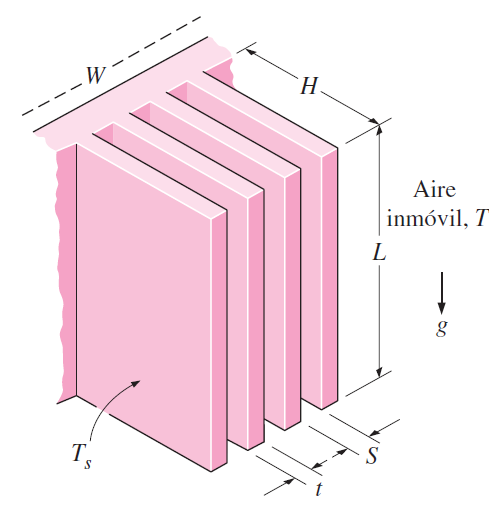
\includegraphics[scale=0.55]{Figuras/ejemplodisipador.png}
\caption{Esquema constructivo de un disipador de calor}
Fuente:\cite{cengel}
\label{ejemplo disipador}
\end{figure}

\begin{equation}\label{sopt}
    S_{opt}=2.714\cdot \frac{L}{Ra_{L}^{0.25}}\;\;(\si{\meter})
\end{equation}

Una vez con el espaciado óptimo se puede determinar el número de aletas para una configuración como la mostrada en la Figura \ref{ejemplo disipador}.

\begin{equation}\label{numeroaletas}
    n=\frac{W}{S+t}
\end{equation}

Cuando el espaciado $S$ es el  óptimo $S_{opt}$ el número de Nusselt es constante con un valor de 1,307; lo que permite determinar también el coeficiente de convección natural. 

\begin{equation}\label{hdisipador}
    Nu=\frac{hS_{opt}}{k}=1.307
\end{equation}

Finalmente para determinar la razón de transferencia de calor se utiliza la Ecuación \ref{Newton}, para el caso de $Ra_{L}$, se utiliza la Ecuación \ref{ra1}, se evaluán las propiedades del aire a $T_{prom}$ (Ecuación \ref{tf}).

\textbf{Refrigeración Pasiva versus Refrigeración Activa:} Se dice que la refrigeración es pasiva cuando la transferencia de calor se realiza de manera natural con los elementos del sistema sin necesidad de mecanismos o trabajo mecánico para acelerar o mejorar el proceso de transferencia, como sí sucede en el caso de la refrigeración activa donde existe un flujo forzado del medio refrigerante. \cite{cengel}

La refrigeración pasiva como no depende de mecanismos que requieren de energía para realizar el trabajo mecánico, así como equipos auxiliares que eventualmente requerirán de mantenimiento, reducen el costo y aumentan la confiabilidad del sistema; sin embargo, presenta la desventaja de ser eficiente para flujos de calor bajos e implica que el elemento a refrigerar opere a temperaturas mas altas. \cite{motor}

\textbf{Control térmico en gabinetes eléctricos:} Cuando se habla de circuitos y tableros eléctricos que se utilizan en múltiples áreas de la industria, se debe considerar que los mismos son susceptibles a diferentes factores que pueden provocar daños en su estructura y componentes; por lo que, actualmente en la industria existen diversas soluciones en forma de gabinetes y racks que aseguran la integridad de sus componentes internos\cite{factores}. Sin embargo, esto representa un reto a nivel térmico el poder mantener en temperaturas operativas a los componentes electrónicos; se estima que por cada \SI{10}{\celsius} por encima de la temperatura de operación del recinto se reduce hasta en un $50\%$ la vida útil del dispositivo electrónico. \cite{hoffman}

Por otro lado la humedad presente en los gabinetes eléctricos representan un riesgo muy grande para la integridad de los componentes internos, y que se podrían producir condensaciones internas debido al flujo de aire húmedo que choca contra superficies con una temperatura por debajo de la de rocío; y provocar daños en componentes electrónicos y posibles focos de corrosión en el gabinete y herrajes. Este problema se presenta principalmente en gabinetes que tiene un sistema de refrigeración robusto en donde el evaporador podría generar condensaciones a lo interno, o bien al realizar aperturas de mantenimiento, el ingreso de aire húmedo caliente con respecto al aire frió interno podría provocar la condensación. \cite{risoul}

Una forma de determinar si la condensación se producirá es mediante la Ecuación \ref{calculo td}  que permite relacionar la temperatura ambiente $T_{amb}$ con el porcentaje de humedad relativa $HR$ para obtener la temperatura de rocío $T_{d}$.\cite{td}

\begin{equation}\label{calculo td}
    T_{d}= c3*\frac{\ln \left ( \frac{RH}{100} \right )+\frac{c2*T_{amb}}{c3+T_{amb}}}{c2-\ln \left ( \frac{RH}{100} \right )-\frac{c2*T_{amb}}{c3+T_{amb}}}
\end{equation}

Para $T\,>0\degree C\;:\;c2=17,08085\;;\;c3=234,175$